% !TEX root = ../main.tex


%[3 p. 90]  
\item\pt{4}\begin{minipage}[t]{.45\linewidth}
Je gooit een bal verticaal omhoog tegen het plafond. De referentie-as staat verticaal omhoog en de grond is de oorsprong. %Hou geen rekening met de versnelling ten gevolge van de botsingen. 
Welk $v(t)$-diagram geeft het best de snelheid van de bal weer? 

\vspace{\baselineskip}
Licht kort toe.
\end{minipage}
\hfill
\begin{minipage}[t]{.5\linewidth}
	\raisebox{1ex-\height}{%
		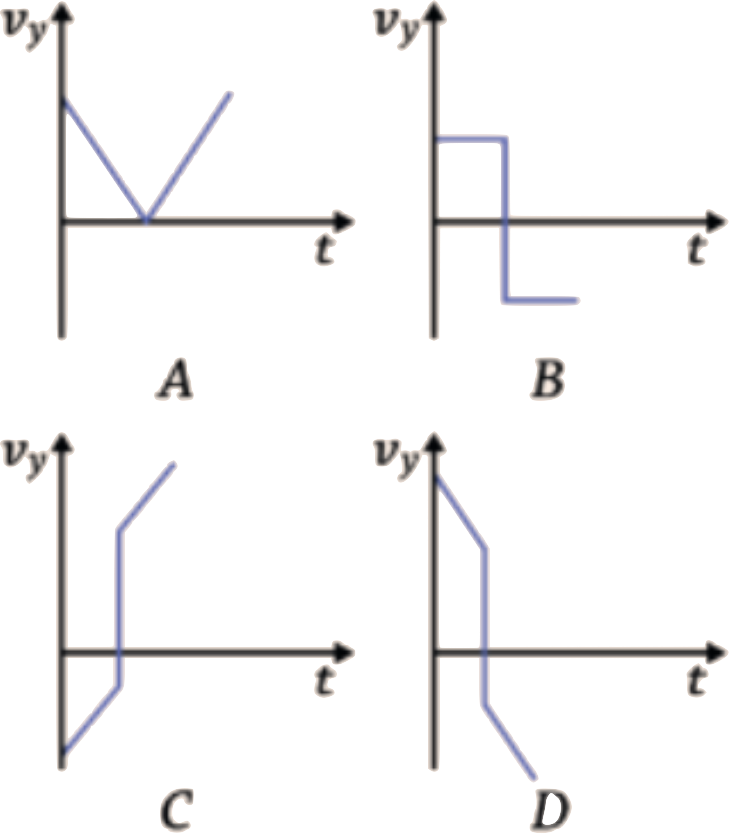
\includegraphics[width=\textwidth]{3p90}} 
\end{minipage}

\begin{oplossing}
D geeft het juiste verloop weer.

Omdat de $y$-as, de as waarmee de beweging beschreven wordt, verticaal omhoog gekozen is, moet de versnellingscomponent negatief zijn. De versnellingsvector is immers naar beneden gericht. De beginsnelheid is met de as mee en dus positief. Omdat de versnelling constant is, moet de snelheid lineair afnemen. Aan deze inzichten voldoen enkel A en D.

Bij de botsing tegen het plafond moet de bal op een hele korte tijd tot stilstand komen om vervolgens op een hele korte tijd weer een even grote snelheid te krijgen, maar nu naar benden. Bij het terug naar beneden komen is de snelheid(svector) tegengesteld gericht aan de as, zodat de component ervan negatief moet zijn. Aan deze beschrijving voldoet enkel D.

\end{oplossing}